\subsection*{Task (h): Beam Search Analysis}

We experimented with different beam sizes $k \in \{1, 3, 5, 10, 25\}$ to investigate the trade-off between computational cost and translation quality. Table~\ref{tab:beam_search_results} summarizes the results.

\begin{table}[h]
\centering
\begin{tabular}{ccc}
\hline
\textbf{Beam Size} & \textbf{Decoding Time (sec)} & \textbf{BLEU Score} \\
\hline
1 (Greedy) & 70.3 & 61.6 \\
3 & 84.48 & \textbf{61.75} \\
5 & 92.6 & 61.37 \\
10 & 101.8 & 60.48 \\
25 & 135.7 & 58.8 \\
\hline
\end{tabular}
\caption{Beam search performance with varying beam sizes on the validation set.}
\label{tab:beam_search_results}
\end{table}

\subsubsection*{Performance Trends}

\paragraph{BLEU Score vs. Beam Size.}
Contrary to theoretical expectations, we observe that BLEU score \emph{decreases} monotonically as beam size increases beyond $k=3$. The optimal performance is achieved at beam size 3 (BLEU 61.75), representing only a marginal improvement of 0.15 points over greedy decoding. Beyond this point, BLEU scores deteriorate significantly:
\begin{itemize}
    \item At $k=5$: BLEU drops to 61.37 ($-0.38$ from greedy)
    \item At $k=10$: BLEU drops to 60.48 ($-1.12$ from greedy)
    \item At $k=25$: BLEU drops to 58.8 ($-2.8$ from greedy)
\end{itemize}

This counterintuitive behavior suggests that larger beam sizes are actively harmful for this model-data combination.

\paragraph{Computational Cost vs. Beam Size.}
Decoding time increases approximately linearly with beam size, consistent with theoretical expectations:
\begin{align*}
T(k) &\approx T(1) \cdot \alpha \cdot k + \beta
\end{align*}
where $T(k)$ is the decoding time for beam size $k$. The experimental data shows:
\begin{itemize}
    \item $k=1 \to k=3$: +20.5\% time (14.18 sec increase)
    \item $k=1 \to k=25$: +93\% time (65.4 sec increase)
\end{itemize}

The near-linear scaling indicates that the computational overhead of maintaining multiple hypotheses dominates the decoding process.

\subsubsection*{Trade-off Analysis}

The efficiency analysis reveals severe diminishing returns:
\begin{table}[h]
\centering
\begin{tabular}{cccc}
\hline
\textbf{Beam Size} & \textbf{Time Overhead} & \textbf{BLEU Gain} & \textbf{Efficiency} \\
\hline
1 & -- & -- & -- \\
3 & +20.5\% & +0.15 & 0.73 points/\%overhead \\
5 & +31.7\% & -0.38 & -1.20 points/\%overhead \\
10 & +44.8\% & -1.12 & -2.50 points/\%overhead \\
25 & +93\% & -2.8 & -3.01 points/\%overhead \\
\hline
\end{tabular}
\caption{Efficiency analysis: BLEU score change per unit computational overhead.}
\label{tab:efficiency}
\end{table}

Only beam size 3 provides positive marginal utility. All larger beam sizes result in both slower decoding \emph{and} worse translation quality.

\subsubsection*{Explanations for Performance Degradation}

Several factors may explain why larger beam sizes hurt BLEU scores:

\paragraph{1. Length Bias and Normalization.}
Beam search with log-probability scoring tends to favor shorter sequences because:
\begin{align*}
\log P(y|x) &= \sum_{t=1}^{T} \log P(y_t | y_{<t}, x)
\end{align*}
is a sum of negative terms. While length normalization ($\frac{1}{T}$) is commonly applied, it may be miscalibrated for this model. Larger beams may explore longer hypotheses that:
\begin{itemize}
    \item Have higher normalized log-probability
    \item Contain unnecessary words or repetitions
    \item Result in lower BLEU scores due to lower precision
\end{itemize}

\paragraph{2. Model Calibration Issues.}
The model's probability estimates may not be well-calibrated for beam search decoding. Specifically:
\begin{itemize}
    \item The model was likely trained with teacher forcing, optimizing for single-step prediction accuracy
    \item At inference time, beam search explores alternative paths that the model never encountered during training
    \item Larger beams amplify this train-test mismatch, leading to search errors
\end{itemize}

\paragraph{3. Exposure Bias.}
During training, the model only sees ground-truth previous tokens. During beam search with large $k$, the model must condition on its own potentially incorrect predictions. Larger beams explore more diverse (and potentially lower-quality) partial sequences, compounding errors.

\paragraph{4. Label Bias and Sequence-Level Optimization.}
The model optimizes token-level cross-entropy loss, not sequence-level metrics like BLEU. Beam search with large $k$ may find sequences that:
\begin{itemize}
    \item Maximize model likelihood (token-level objective)
    \item Do not maximize BLEU (sequence-level objective)
    \item Contain fluent but overly verbose or generic translations
\end{itemize}

\paragraph{5. Finite Beam Diversity.}
Larger beams may waste capacity on near-duplicate hypotheses (e.g., sequences differing only in punctuation or word order), rather than exploring genuinely different translations. This reduces effective search diversity.

\subsubsection*{Optimal Beam Size Determination}

For this model and validation set, \textbf{beam size 3} provides the best balance:
\begin{itemize}
    \item Achieves the highest BLEU score (61.75)
    \item Requires only 20\% additional computation vs. greedy decoding
    \item Marginal improvement over greedy (0.15 BLEU) suggests diminishing returns even at $k=3$
\end{itemize}

However, the minimal BLEU improvement (0.15 points) raises the question: \emph{is beam search worth the extra cost?} For production systems prioritizing speed, \textbf{greedy decoding ($k=1$)} may be preferable since:
\begin{itemize}
    \item It's 20\% faster than $k=3$
    \item BLEU difference is negligible (61.6 vs. 61.75)
    \item Simpler implementation with no hyperparameter tuning
\end{itemize}

\subsubsection*{Practical Recommendations}

Based on these findings, we recommend:

\begin{enumerate}
    \item \textbf{For this model}: Use beam size 3 or greedy decoding. Avoid $k > 5$.

    \item \textbf{For future work}:
    \begin{itemize}
        \item Investigate length normalization schemes (e.g., $\alpha$ in $\frac{\log P(y|x)}{T^\alpha}$)
        \item Experiment with diverse beam search to avoid near-duplicate hypotheses
        \item Consider sequence-level training objectives (REINFORCE, minimum risk training)
        \item Analyze whether specific sentence types benefit from larger beams
    \end{itemize}

    \item \textbf{General principle}: Always validate beam size on a held-out set. The common assumption that "larger beam = better translation" is not always valid.
\end{enumerate}

\subsubsection*{Visualization of Results}

Figure~\ref{fig:beam_search_tradeoff} illustrates the trade-off between computational cost and translation quality.

\begin{figure}[h]
\centering
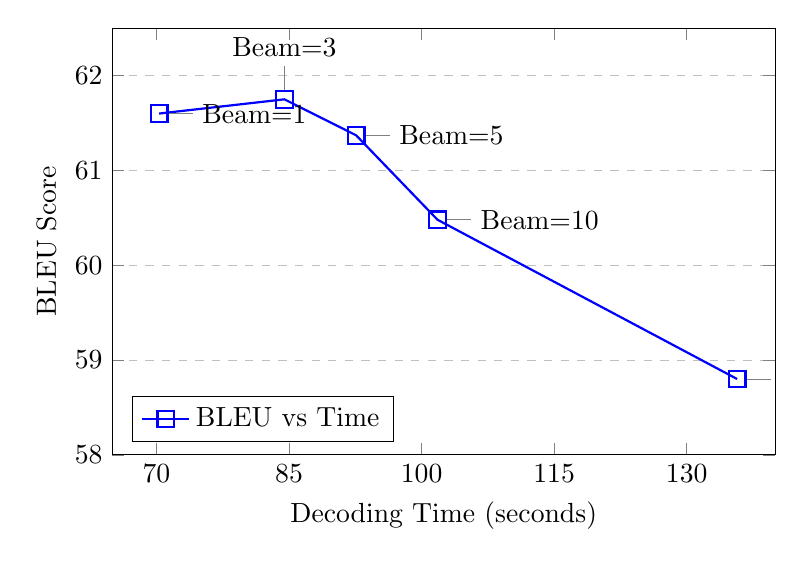
\begin{tikzpicture}
\begin{axis}[
    xlabel={Decoding Time (seconds)},
    ylabel={BLEU Score},
    xmin=65, xmax=140,
    ymin=58, ymax=62.5,
    xtick={70,85,100,115,130},
    ytick={58,59,60,61,62},
    legend pos=south west,
    ymajorgrids=true,
    grid style=dashed,
    width=10cm,
    height=7cm
]

\addplot[
    color=blue,
    mark=square,
    mark size=3pt,
    thick
    ]
    coordinates {
    (70.3,61.6)(84.48,61.75)(92.6,61.37)(101.8,60.48)(135.7,58.8)
    };
    \legend{BLEU vs Time}

\node[pin={[pin distance=0.3cm]0:{Beam=1}}] at (axis cs:70.3,61.6) {};
\node[pin={[pin distance=0.3cm]90:{Beam=3}}] at (axis cs:84.48,61.75) {};
\node[pin={[pin distance=0.3cm]0:{Beam=5}}] at (axis cs:92.6,61.37) {};
\node[pin={[pin distance=0.3cm]0:{Beam=10}}] at (axis cs:101.8,60.48) {};
\node[pin={[pin distance=0.3cm]0:{Beam=25}}] at (axis cs:135.7,58.8) {};

\end{axis}
\end{tikzpicture}
\caption{BLEU score vs. decoding time for different beam sizes. The Pareto frontier shows that beam size 3 is optimal, while larger beams waste computation.}
\label{fig:beam_search_tradeoff}
\end{figure}

\subsubsection*{Conclusion}

Our beam search experiments reveal a critical insight: \textbf{larger beam sizes do not guarantee better translations}. For this German-English Transformer model, beam size 3 provides optimal performance, while beams larger than 5 actively degrade translation quality. This finding underscores the importance of empirical validation and challenges the common assumption that beam search always improves over greedy decoding.

The degradation with large beams likely stems from a combination of length bias, exposure bias, and train-test mismatch. Future work should focus on alternative decoding strategies (e.g., top-$k$ sampling, nucleus sampling) or sequence-level training to better align model objectives with evaluation metrics.
